\documentclass{beamer}

\usepackage[brazil]{babel}
\usepackage[T1]{fontenc}
\usepackage[utf8]{inputenc}

\usepackage{listings}

\usepackage{hyperref}
\hypersetup{
    colorlinks=true,
    linkcolor=blue,
    urlcolor=red,
}

\usepackage{multicol}

\usetheme{Hannover}
\usecolortheme{crane}

\newcommand{\lang}[1]{\texttt{#1}}
\newcommand{\inlcode}[1]{\texttt{#1}}

\newcommand{\nota}[1]{\textbf{Nota:}\textit{ #1}}

\renewcommand{\d}{\:.\:}

% Tipos {
\newcommand{\typetam}{\#}
\newcommand{\typeeq}{\equiv}
\newcommand{\typesim}{\simeq}
% }

\newcommand{\tabelasizealign}{%
    \begin{tabular}{|c|c|c|}%
        \hline%
        Tipo & sizeof & alignment \\\hline%
        \hline%
        bool & 1      & 1         \\\hline%
        u32  & 4      & 4         \\\hline%
        u64  & 8      & 8         \\\hline%
    \end{tabular}%
}

\newcommand{\tabelasizealignTwo}{%
    \begin{tabular}{|c|c|c||c|c|c|}%
        \hline%
        Tipo & sizeof & alignment &%
        Tipo & sizeof & alignment \\\hline%
        \hline%
        bool & 1      & 1         &%
        u32  & 4      & 4         \\\hline&&&%
        u64  & 8      & 8         \\\hline%
    \end{tabular}%
}

\title{Tipos do Céu ao Chão}
\author{Hashimoto}
\date{22 de Junho de 2022}

\begin{document}

\begin{frame}
    \titlepage
\end{frame}

\begin{frame}
    \frametitle{Meme}
    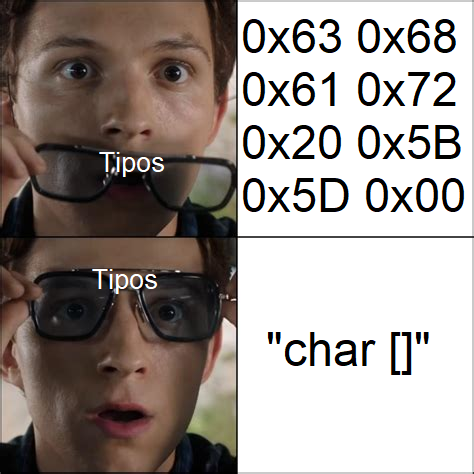
\includegraphics[height=.85\textheight,angle=0]{char_meme.png}
    \centering
\end{frame}

\begin{frame}
    \frametitle{ToC}
    \tableofcontents[hideallsubsections]
\end{frame}

\section{Tipos}
\begin{frame}
    \frametitle{Intro}
\end{frame}

\begin{frame}
    \frametitle{Notação}
    Alto nível:
    \begin{itemize}
        \item Tamanho de um tipo: \(\typetam(A)\)
        \item Dois tipos são iguais: \( A \typeeq B \)
        \item Dois tipos são isomorficos (equivalentes):
            \( A \typesim B \)
        \item Função que recebe \(A\), \(B\), \(C\),
            e retorna \(D\): \[ A \to B \to C \to D \]
    \end{itemize}

    Baixo nível:
    \begin{itemize}
        \item Inteiro com sinal de \(n\) bits: \(i\_n\)
        \item Inteiro com sinal de \(32\) bits: \(i32\)
        \item Inteiro sem sinal de \(n\) bits: \(u\_n\)
        \item Inteiro sem sinal de \(32\) bits: \(u32\)
        \item Booleano de tamanho byte: \(bool\)
            \\\nota{\(bool \typesim u1\)}
    \end{itemize}
\end{frame}

\section{Tipos - Caso Recursivo}
\begin{frame}
    \frametitle{Caso Recusivo}
    O ``caso recursivo'' é para criar \emph{tipos novos}.
    \vfill
    Para \emph{usar} os tipos novos,
    precisamos de formas (funções) para:
    \begin{itemize}
        \item definir/criar novos elementos
            (\emph{construtores})
        \item transformar os elementos já definidos:
            (\emph{destrutores})
    \end{itemize}
    \vfill
    \nota{Em lógica, os \emph{construtores}
        são chamados de \emph{regras de introdução} e
        os \emph{destrutores}
        de \emph{regras de eliminação}}
\end{frame}

\subsection{Produto}
\begin{frame}
    \frametitle{Produto \(A \times B\)}
    \begin{itemize}
        \item Construtor
            \[
                A \to B \to A \times B
            \]
            \vfill
        \item Destrutor (projeções)
            \[
                \pi_A : A \times B \to A
            \] \[
                \pi_B : A \times B \to B
            \]
            \vfill
        \item Valores
            \[
                \typetam(A \times B) = \typetam(A) \times \typetam(B)
            \]
    \end{itemize}
\end{frame}

\begin{frame}
    \frametitle{Corolário}
    \begin{itemize}
        \item É associativo:
            \[
                (A \times B) \times C \typesim A \times (B \times C)
            \]
            \vfill
        \item É comutativo:
            \[
                (A \times B) \typesim (B \times A)
            \]
    \end{itemize}
\end{frame}

\begin{frame}[fragile]
    \frametitle{Exemplos: \(A \times B\)}
    \begin{itemize}
        \item \lang{C} \emph{(Struct)}:
            \begin{lstlisting}[language=C]
struct ProdutoIntDouble {
    int a;
    double b;
};
            \end{lstlisting}
        \item \lang{Java} \emph{(Class/Object)} (*):
            \begin{lstlisting}[language=Java]
class ProdutoIntDouble {
    private int a;
    private double b;
}
            \end{lstlisting}
        \item \lang{Haskell} \emph{(Record)}:
            \begin{lstlisting}[language=Haskell]
data ProdutoIntDouble = PIntDouble
    { a :: Int
    , b :: Double
    }
            \end{lstlisting}
    \end{itemize}
\end{frame}

\begin{frame}
    \frametitle{Matemática de Struct}
    Informações importantes de uma \emph{struct}:
    \begin{itemize}
        \item Tamanho \emph{(sizeof)}:
            quantos bytes ocupa?
        \item Alinhamento \emph{(alignment)}:
            endereço é múltiplo de quanto?
    \end{itemize}
    \vfill
    \nota{Nem sempre o \emph{tamanho final}
        é a soma dos \emph{tamanhos}!}
    \vfill
    Alinhamento:
    \url{www.delftstack.com/howto/c/struct-alignment-in-c/}
\end{frame}

\begin{frame}[fragile]
    \frametitle{Exemplos: Matemática de Struct}
    \begin{multicols}{2}
        \begin{lstlisting}[language=C]
struct Exemplo1 {
    u32 a;
    u32 b;
};
        \end{lstlisting}
        \begin{lstlisting}[language=C]
struct Exemplo2 {
    u32 a;
    bool b;
};
        \end{lstlisting}
        \begin{lstlisting}[language=C]
struct Exemplo3 {
    u64 a;
    u32 b;
    u32 c;
};
        \end{lstlisting}
        \columnbreak
        \begin{lstlisting}[language=C]
struct Exemplo4 {
    u32 b;
    u64 a;
    u32 c;
};
        \end{lstlisting}
        \begin{lstlisting}[language=C]
struct Exemplo5 {
    u32 b; u32 pad1;
    u64 a;
    u32 c; u32 pad2;
};
        \end{lstlisting}
        \tabelasizealign{}
    \end{multicols}
\end{frame}

\begin{frame}
    \frametitle{Respostas: Matemática de Struct}
    \begin{center} \begin{tabular}{|c|c|c||c|}
        \hline%
        Tipo      & sizeof & alignment & waste \\\hline
        \hline
        bool      & 1      & 1         & 0     \\\hline
        u32       & 4      & 4         & 0     \\\hline
        u64       & 8      & 8         & 0     \\\hline
        \hline
        Exemplo1  & 8      & 4         & 0     \\\hline
        Exemplo2  & 8      & 4         & 3     \\\hline
        Exemplo3  & 16     & 8         & 0     \\\hline
        Exemplo4  & 24     & 8         & 8     \\\hline
        Exemplo5  & 24     & 8         & 0     \\\hline
    \end{tabular} \end{center}
\end{frame}

\subsection{Soma}
\begin{frame}
    \frametitle{Soma \(A + B\)}
    \begin{itemize}
        \item Construtores
            \[
                left : A \to A + B
            \] \[
                right : B \to A + B
            \]
            \vfill
        \item (Família de) Destrutor(es)
            \[
                \forall X \d
            \] \[
                A + B \to (A \to X) \to (B \to X) \to X
            \]
            \vfill
        \item Valores
            \[
                \typetam(A + B) = \typetam(A) + \typetam(B)
            \]
            \vfill
        \item Outros nomes: Coproduto, Variante
    \end{itemize}
\end{frame}

\begin{frame}
    \frametitle{Corolário}
    \begin{itemize}
        \item É associativo:
            \[
                (A + B) + C \typesim A + (B + C)
            \]
            \vfill
        \item É comutativo:
            \[
                (A + B) \typesim (B + A)
            \]
    \end{itemize}
\end{frame}

\begin{frame}[fragile]
    \frametitle{Unions}
    Em \lang{C}, temos \emph{Unions}!
    \vfill
    \begin{multicols}{2}
        \begin{lstlisting}[language=C]
union quase_soma {
    int a;
    float b;
    char c;
};
        \end{lstlisting}
        \columnbreak
        \nota{Depois que criamos um elemento da \inlcode{union}
        perdemos a informação de qual caso ele representa!}
    \end{multicols}
    \vfill
    Isso aloca um espaço na memória que pode armazenar
    um \inlcode{int} ou(-exclusivo)
    um \inlcode{float} ou(-exclusivo)
    um \inlcode{char}.
    \vfill
    O \emph{sizeof} é o
    \(\max(sizeof(int), sizeof(float), sizeof(char))\).
    \\
    O \emph{alignment} é o
    \(\max(align(int), align(float), align(char))\).
\end{frame}

\begin{frame}[fragile]
    \frametitle{Enums}
    Em \lang{C}, também temos \emph{Enums}!
    \vfill
    \begin{lstlisting}[language=C]
enum casos_soma {
    CASO_SOMA_A, CASO_SOMA_B, CASO_SOMA_C,
};
    \end{lstlisting}
    \vfill
    Isso dá ``um nome'' para alguns inteiros de \(0\) até \(2^n-1\)
    (em \lang{C} \(n := 32\),
    mas a princípio pode ser qualquer potência de \(2\))
    \vfill
    O \emph{sizeof} é o \(sizeof(un)\)
    (no caso do \lang{C} é \(sizeof(u32)\)).
    \\
    O \emph{alignment} é o \(align(un)\)
    (no caso do \lang{C} é \(align(u32)\)).
\end{frame}

\begin{frame}[fragile]
    \frametitle{Tagged Unions}
    Agora podemos juntar as duas!
    \vfill
    \begin{lstlisting}[language=C]
enum casos_soma {
    CASO_SOMA_A, CASO_SOMA_B, CASO_SOMA_C,
};

union quase_soma {
    int a; float b; char c;
};

struct soma {
    union quase_soma as;
    enum casos_soma tag;
};
    \end{lstlisting}
\end{frame}

\begin{frame}[fragile]
    \frametitle{Tagged Unions}
    Equivalente!
    \vfill
    \begin{lstlisting}[language=C]
struct soma {
    union quase_soma {
        int a; float b; char c;
    } as;

    enum casos_soma {
        CASO_SOMA_A, CASO_SOMA_B,
        CASO_SOMA_C,
    } tag;
};
    \end{lstlisting}
\end{frame}

\begin{frame}
    \frametitle{Matemática de Tagged Union}
    No fim, uma \inlcode{Tagged Union} é só
    uma \inlcode{struct} de
    um \inlcode{enum} e uma \inlcode{union}.
\end{frame}

\begin{frame}[fragile]
    \frametitle{Exemplos: Matemática de Tagged Union}
    \begin{lstlisting}[language=C]
struct Exemplo1 {
    union { u32 a; u64 b; } as;
    enum { CASO_U32, CASO_U64, } tag; };
    \end{lstlisting}
    \begin{lstlisting}[language=C]
struct Exemplo2 {
    union { u32 a; u64 b; bool c; } as;
    enum { C_U32, C_U64, C_BOOL, } tag; };
    \end{lstlisting}
    \begin{lstlisting}[language=C]
struct Exemplo3 {
    union { u32 a; u32 b; u32 c; u32 d;
        u32 e; u32 f; u32 g; u32 h; } as;
    enum { A, B, C, D, E, F, G, H, } tag; };
    \end{lstlisting}
    \tabelasizealignTwo{}
\end{frame}

\begin{frame}
    \frametitle{Respostas: Matemática de Tagged Union}
    \begin{center} \begin{tabular}{|c|c|c|}
        \hline%
        Tipo      & sizeof & alignment \\\hline
        \hline
        bool      & 1      & 1         \\\hline
        u32       & 4      & 4         \\\hline
        u64       & 8      & 8         \\\hline
        \hline
        Exemplo1  & 16     & 8         \\\hline
        Exemplo2  & 16     & 8         \\\hline
        Exemplo3  & 8      & 4         \\\hline
    \end{tabular} \end{center}
\end{frame}

\begin{frame}[fragile]
    \frametitle{Exemplos: \(A + B\)}
    \begin{itemize}
        \item \lang{Zig} \emph{(Tagged Union)}:
            \begin{lstlisting}[language=C]
const UnionIntDouble = union(enum) {
    caso_int: u32,
    caso_double: f64,
};
            \end{lstlisting}
    \end{itemize}
\end{frame}

\begin{frame}[fragile]
    \frametitle{Exemplos: \(A + B\)}
    \begin{itemize}
        \item \lang{Java} \emph{(Inheritance/Dynamic Dispatch)} (*):
            \begin{lstlisting}[language=Java]
abstract class UnionBase {}

class UnionInt extends UnionBase {
    private int val;
}

class UnionDouble extends UnionBase {
    private double val;
}
            \end{lstlisting}
    \end{itemize}
\end{frame}

\begin{frame}[fragile]
    \frametitle{Exemplo Bônus: \(A + B\)}
    \begin{itemize}
        \item Algo parecido em \lang{C}
            \emph{(``Struct Inheritance'')}:
            \begin{lstlisting}[language=C]
enum UnionTag { CASO_INT, CASO_DOUBLE };

struct UnionHeader {
    enum UnionTag tag;
}

struct UnionInt {
    struct UnionHeader header;
    int val;
}

struct UnionDouble {
    struct UnionHeader header;
    double val;
}
            \end{lstlisting}
    \end{itemize}
\end{frame}

\begin{frame}[fragile]
    \frametitle{Exemplos: \(A + B\)}
    \begin{itemize}
        \item \lang{Rust} \emph{(Enum)}:
            \begin{lstlisting}[language=C]
enum UnionIntDouble {
    CasoInt(i32),
    CasoDouble(f64)
}
            \end{lstlisting}
            \vfill
        \item \lang{Haskell} \emph{(Algebraic Data Type)}:
            \begin{lstlisting}[language=Haskell]
data UnionIntDouble
    = CasoInt Int
    | CasoDouble Double
            \end{lstlisting}
    \end{itemize}
\end{frame}

\subsection{Exponencial}
\begin{frame}
    \frametitle{Exponencial \(B^A\)}
    \begin{itemize}
        \item Construtor
            \[
                (A \to B) \to B^A
            \]
            \vfill
        \item Destrutor
            \[
                eval : B^A \to A \to B
            \]
            \vfill
        \item Valores
            \[
                \typetam\left(B^A\right) = \typetam(B)^{\typetam(A)}
            \]
    \end{itemize}
\end{frame}

\begin{frame}
    \frametitle{Corolário}
    \begin{itemize}
        \item \textbf{Não} é associativo:
            \[
                \left(A^B\right)^C \not\typesim A^{\left(B^C\right)}
            \]
            \vfill
        \item \textbf{NÃO} é comutativo:
            \[
                \left(A^B\right) \not\typesim \left(B^A\right)
            \]
    \end{itemize}
\end{frame}

\begin{frame}
    \frametitle{Exponencial \(B^A\)}
    Opções de implementação:
    \begin{itemize}
        \item Look-up Table (Arrays)
            \begin{itemize}
                \item Memória:
                    \(sizeof(B) \times \typetam(A)\)
                    \par
                    \nota{Precisa converter \(A\) para inteiro}
            \end{itemize}
        \vfill
        \pause
        \item Ponteiros para função:
            \begin{itemize}
                \item Memória:
                    \emph{código} (estático)
                    + \emph{ponteiro} (cada instância)
            \end{itemize}
        \vfill
        \pause
        \item (Código de uma) Máquina Virtual
        \vfill
        \pause
        \item ??? (Céu é o limite)
    \end{itemize}
\end{frame}

\begin{frame}
    \frametitle{Por que \(B^A\)?}
    Um grande motivo é \emph{Programação Funcional}:
    \begin{itemize}
        \item Receber/Passar uma função
        \item Closures
        \item Aplicação Parcial
        \item Callbacks
    \end{itemize}
    \vfill
    \pause
    Também serve como base para
    \emph{Virtual Tables} \emph{(Vtables)}:
    \begin{itemize}
        \item Intefaces
        \item Dynamic Dispatch
    \end{itemize}
\end{frame}

\section{Tipos - Casos Base}
\begin{frame}
    \frametitle{Caso Base}
    \begin{itemize}
        \item Aqui ficam os \emph{tipos primitivos/atômicos}
            \vfill
        \item Não dá para quebrar mais que isso!
            \vfill
        \item Também têm \emph{contrutores} e \emph{destrutores}
    \end{itemize}
\end{frame}

\subsection{Void}
\begin{frame}
    \frametitle{\(Void\)}
    \only<1>{
        Pausa Dramática!
        \centering
    } \only<2-> {
        \begin{itemize}
            \item Construtor
                \[
                    \text{(não tem)}
                \]
                \vfill
            \item Destrutor
                \[
                    \forall X \d
                \] \[
                    absurd : Void \to X
                \]
                \vfill
            \item Valores
                \[
                    0
                \]
                \vfill
            \item \nota{Em lógica, é o \(\bot\) \emph{(false)}}
        \end{itemize}
    }
\end{frame}

\subsection{Unity}
\begin{frame}
    \frametitle{Unity -- \(()\)}
    \begin{itemize}
        \item Construtor
            \[
                () : ()
            \]
            \vfill
        \item Destrutor
            \[
                \text{(não tem)}
            \]
            \vfill
        \item Valores
            \[
                1
            \]
            \vfill
        \item \nota{Em lógica, é o \(\top\) \emph{(true)}}
    \end{itemize}
\end{frame}

\begin{frame}[fragile]
    \frametitle{\inlcode{void} \(== ()\)}
    Se ``\inlcode{void} \(== ()\)'',
    por que eu não posso fazer isso:
    \vfill
    \begin{lstlisting}[language=C]
void func(void) {}

int main() {
    void v;
    v = func();
}
    \end{lstlisting}
\end{frame}

\begin{frame}[fragile]
    \frametitle{\inlcode{void} \(== ()\)}
    \begin{lstlisting}
> gcc a.c
a.c: In function 'main':
a.c:4:10: error: variable or field
'v' declared void
    4 |     void v;
      |          ^
a.c:5:7: error: void value not ignored
as it ought to be
    5 |     v = func();
      |
    \end{lstlisting}
\end{frame}

\begin{frame}[fragile]
    \frametitle{\inlcode{void} \(== ()\)}
    Em \lang{Zig}, pode!
    \vfill
    \begin{lstlisting}[language=C]
fn func() void {}

pub fn main() u8 {
    var v: void = undefined;
    v = func();
    return 0;
}
    \end{lstlisting}
\end{frame}

\subsection{Bool}
\begin{frame}
    \frametitle{Bool}
    \begin{itemize}
        \item Construtor
            \[
                false : Bool
            \] \[
                true : Bool
            \]
            \vfill
        \item (Família de) Destrutor(es)
            \[
                \forall X \d
            \] \[
                Bool \to X \to X \to X
            \]
            \vfill
        \item Valores
            \[
                2
            \]
    \end{itemize}
\end{frame}

\begin{frame}
    \frametitle{Bool \(\typesim () + ()\)}
    Se a gente usar a Soma \(() + ()\):
    \vfill
    \begin{itemize}
        \item Construtores
            \[
                left : () \to () + ()
            \] \[
                right : () \to () + ()
            \]
            \vfill
        \item (Família de) Destrutor(es)
            \[
                \forall X \d
            \] \[
                () + () \to (() \to X) \to (() \to X) \to X
            \]
            \vfill
        \item Valores
            \[
                \typetam(() + ()) = \typetam(()) + \typetam(())
                = 2
            \]
            \vfill
        \item Só chamar \(left\) de \inlcode{false} e
            \(right\) de \inlcode{true} (ou o oposto)!
    \end{itemize}
    \vfill
    \nota{Acredita em mim que \(A \typesim () \to A\)}
\end{frame}

\subsection{Int}
\begin{frame}
    \frametitle{I32}
    Vocês lembram da representação binária de um \inlcode{I32}?
    \vfill
    \begin{align*}
        I32 &\typesim Bool \times Bool \times \cdots \times Bool \\
        &\typesim (()+()) \times \cdots \times (()+()) \\
        &\typesim () + () + () + \cdots + () + () \\
    \end{align*}
    \vfill
    Então dá para representar \emph{muita coisa} usando
    só \emph{Produto, Soma e Unity}.
    \vfill
    Mas isso não quer dizer que
    a gente deva usar essas representações!
    O hardware sabe trabalhar muito bem com \inlcode{I32},
    então faz sentido ele ser um tipo primitivo.
\end{frame}

\subsection{Tipos Algébricos}
\begin{frame}[fragile]
    \frametitle{Tipos Algébricos}
    Deveria estar em \textbf{Tipos - Caso Recursivo},
    mas se encaixa melhor aqui!
    \vfill
    \emph{Tipos Algébricos}
    é uma forma para representar somas e produtos:
    \vfill
    \begin{lstlisting}[language=Haskell]
Bool = False | True
    \end{lstlisting}
    \vfill
    \begin{lstlisting}[language=Haskell]
I32_1 = I32_1 Bool Bool Bool ... Bool
    \end{lstlisting}
    \vfill
    \begin{lstlisting}[language=Haskell]
I32_2 = Int32Min | ... | MenosUm
      | Zero | Um | ... | Int32Max
    \end{lstlisting}
\end{frame}

\section{Polimorfismo Paramétrico}
\begin{frame}
    \frametitle{Polimorfismo}
    \begin{itemize}
        \item Do grego: \emph{muitas formas}
            \vfill
        \item Em programação, geralmente é uma forma
            de permitir que várias coisas diferentes
            exerçam o mesmo papel.
            \vfill
        \item Exemplos:
            \begin{itemize}
                \item Herança
                \item Overloading
                \item \dots
            \end{itemize}
            \vfill
        \item Isso é bem legal,
            pois evita que a gente escreva
            ``duas coisas iguais''.
    \end{itemize}
\end{frame}

\begin{frame}
    \frametitle{Polimorfismo Paramétrico}
    Algumas funções/tipos usam algum tipo já existente
    mas não precisam saber nada sobre esse tipo.
    \vfill
    Outros nomes:
    \begin{itemize}
        \item Generics [Java]
        \item Macros (*) [C]
        \item Meta Programming (Comptime) [Zig]
        \item Templates (typename) [C++]
    \end{itemize}
\end{frame}

\begin{frame}
    \frametitle{Polimorfismo Paramétrico}
    Tipos  que guardam/organizam ``coisas''
    (estruturas de dados) geralmente usam
    muito bem esse tipo de polimorfismo.
    Exemplos: Lista, Fila, Árvore, Mapa, \dots
    \vfill
    Notação para tipos paramétricos:
    \[
        [] : \forall x \d List \; x
    \]
    \vfill
    Notação para essas funções paramétricos:
    \[
        id : \forall x \d x \to x
    \]
    \vfill
    \nota{Geralmente usam letra minúscula para variáveis de tipo}
\end{frame}

\begin{frame}
    \frametitle{Simplificando Destrutores}
    Esse polimorfismo simplifica alguns destrutores,
    onde tinha ``família de destrutores''
    agora é só uma função genérica:
    \begin{itemize}
        \item \(A \times B\)
            \[
                \forall x \d A \times B \to (A \to B \to x) \to x
            \]
        \item \(A + B\)
            \[
                \forall x \d A + B \to (A \to x) \to (B \to x) \to x
            \]
        \item \(Void\)
            \[
                absurd: \forall x \d Void \to x
            \]
        \item \(Bool\)
            \[
                \forall x \d Bool \to x \to x \to x
            \]
    \end{itemize}
\end{frame}

\subsection{Maybe}
\begin{frame}[fragile]
    \frametitle{Maybe a}
    Outros nomes:
    \begin{itemize}
        \item Option
        \item Optional
    \end{itemize}
    \vfill
    \begin{lstlisting}[language=Haskell]
data Maybe a
    = None
    | Some a
    \end{lstlisting}
    \vfill
    Destrutor
    \begin{lstlisting}[language=Haskell]
maybe :: Maybe a -> b -> (a -> b) -> b
maybe  None    b _ = b
maybe (Some a) _ f = f a
    \end{lstlisting}
\end{frame}

\subsection{Either}
\begin{frame}[fragile]
    \frametitle{Either a b}
    Outros nomes:
    \begin{itemize}
        \item Result
        \item Error Union
    \end{itemize}
    \vfill
    \begin{lstlisting}[language=Haskell]
data Either a b
    = Left a
    | Right b
    \end{lstlisting}
    \vfill
    Destrutor
    \begin{lstlisting}[language=Haskell]
either :: Either a b -> (a -> c)
    -> (b -> c) -> c
either (Left  a) f _ = f a
either (Right b) _ g = g b
    \end{lstlisting}
\end{frame}

\subsection{List}
\begin{frame}[fragile]
    \frametitle{List a}
    \begin{lstlisting}[language=Haskell]
data List a
    = Nil
    | Cons a (List a)
    \end{lstlisting}
    \vfill
    Destrutor
    \begin{lstlisting}[language=Haskell]
list :: List a -> b -> (a -> List a -> b)
    -> b
list  Nil        b _ = b
list (Cons a as) _ f = f a as
    \end{lstlisting}
\end{frame}

\begin{frame}[fragile]
    \frametitle{int *p = \&i;}
    \begin{lstlisting}[language=Haskell]
Pointer a = Null
    | Estrela  a
    | Colchete [a]
    \end{lstlisting}
    \vfill
    Problemas (teóricos) dessa representação:
    \begin{itemize}
        \item
            \texttt{C} não sabe diferenciar
            \texttt{Estrela} e \texttt{Colchete}
        \item
            Temos que checar se é \texttt{Null} o tempo todo
        \item
            \textbf{Invisível:} no caso \texttt{Colchete},
            podemos não saber o tamanho da lista
            \par
            \nota{ainda podemos ter o ``null terminator''
            ou guardar um tamanho externo}
        \item
            Na prática, só queremos usar
            \texttt{Estrela} ou \texttt{Colchete}
            \par
            \nota{o ``ou'' é exclusivo}
        \item
            Mais alguns (específicos sobre implementação) \dots
    \end{itemize}
\end{frame}

\begin{frame}[fragile]
    \frametitle{Soluções: Zig}
    \begin{lstlisting}[language=C]
const OptionalInt = ?i32;

const PtrToOneInt = *i32;

const PtrToManyInt = [*]i32;

const NullablePtrToOneInt = ?*i32;

const PtrToOneOptionalInt = *?i32;

const NullablePtrToManyInt = ?[*]i32;

const PtrToManyOptionalInt = [*]?i32;
    \end{lstlisting}
\end{frame}

\begin{frame}[fragile]
    \frametitle{Outros: Zig}
    \begin{lstlisting}[language=C]
// struct { len : usize, data : [*]i32, };
const Slice = []i32;

// Tem valores no array ate achar um A
// A eh um valor de i32
const Sentinel = [*:A]i32;

const CharStar = [*:0]u8;
    \end{lstlisting}
\end{frame}

\begin{frame}
    \frametitle{Implementação (Polimorfismo Paramétrico)}
    \begin{itemize}
        \item Especialização/\emph{inline}:
            \begin{itemize}
                \item Gerar várias funções (\emph{name mangling})
                \item Tudo se resolve estaticamente
                \item Tende a gerar binários maiores
                    (uma função para cada tipo)
            \end{itemize}
            \vfill
        \item \inlcode{void *} e \emph{meta-dados}
            \begin{itemize}
                \item Gerar só uma função
                \item Tudo se resolve dinamicamente
                \item Tende a gerar funções mais lentas
                    (tem que olhar os meta-dados)
            \end{itemize}
    \end{itemize}
\end{frame}

\begin{frame}[fragile]
    \frametitle{Exemplo: Especialização \inlcode{i32}}
    \begin{multicols}{2}
        \begin{lstlisting}[language=C]
struct<T> Pilha {
    usize len;
    usize size;
    [*]T items;
}

Pilha<T> new<T>() {
    return
        Pilha<T> {
    .len = 0,
    .size = 0,
    .items = malloc(
        0*sizeof(T)
        ), };
}
        \end{lstlisting}
        \columnbreak
        \begin{lstlisting}[language=C]
struct Pilha_i32 {
    usize len;
    usize size;
    [*]i32 items;
}

Pilha_i32 new_i32() {
    return
        Pilha_i32 {
    .len = 0,
    .size = 0,
    .items = malloc(
        0*sizeof(i32)
        ), };
}
        \end{lstlisting}
    \end{multicols}
\end{frame}

\begin{frame}[fragile]
    \frametitle{Exemplo: Especialização \inlcode{i32}}
    \begin{lstlisting}[language=C]
void push<T>(Pilha<T> *p, T item) {
    if ( p.size + 1 >= p.len ) {
        p.len *= 2;
        realloc(&p.items, p.len*sizeof(T));
    }
    p.items[p.size] = item;
    p.size += 1;
}
    \end{lstlisting}
    \vfill
    \begin{lstlisting}[language=C]
void push_i32(Pilha_i32 *p, i32 item) {
    if ( p.size + 1 >= p.len ) {
        p.len *= 2;
        realloc(&p.items, p.len*sizeof i32);
    }
    p.items[p.size] = item;
    p.size += 1;
}
    \end{lstlisting}
\end{frame}

\begin{frame}[fragile]
    \frametitle{Exemplo: Especialização \inlcode{i32}}
    \begin{lstlisting}[language=C]
?T pop<T>(Pilha<T> *p) {
    if ( p.size > 0 ) {
        p.size -= 1;
        return p.items[p.size];
    } else return null;
}
    \end{lstlisting}
    \vfill
    \begin{lstlisting}[language=C]
?i32 pop_i32(Pilha_i32 *p) {
    if ( p.size > 0 ) {
        p.size -= 1;
        return p.items[p.size];
    } else return null;
}
    \end{lstlisting}
\end{frame}

\begin{frame}[fragile]
    \frametitle{Exemplo: Generalização}
    \begin{multicols}{2}
        \begin{lstlisting}[language=C]
struct<T> Pilha {
    usize len;
    usize size;
    [*]T items;
}

Pilha<T> new<T>() {
    return Pilha<T> {
    .len = 0,
    .size = 0,
    .items = malloc(
        0*sizeof(T)
        ), };
}
        \end{lstlisting}
        \columnbreak
        \begin{lstlisting}[language=C]
struct Pilha {
    usize len, size;
    Info info;
    [*]*void items;
}

Pilha new(Info i) {
    return Pilha {
    .len =0, .size=0,
    .info = i,
    .items = malloc(
    0*sizeof(*void)
        ), };
}
        \end{lstlisting}
    \end{multicols}
\end{frame}

\begin{frame}[fragile]
    \frametitle{Exemplo: Generalização}
    \begin{lstlisting}[language=C]
void push<T>(Pilha<T> *p, T item) {
    if ( p.size + 1 >= p.len ) {
        p.len *= 2;
        realloc(&p.items, p.len*sizeof(T));
    } p.items[p.size] = item;
    p.size += 1;
}
    \end{lstlisting}
    \vfill
    \begin{lstlisting}[language=C]
void push(Pilha *p, void *item) {
    if ( p.size + 1 >= p.len ) {
        p.len *= 2;
        realloc(&p.items,
            p.len*sizeof(*void));
    }
    p.items[p.size] = item;
    p.size += 1;
}
    \end{lstlisting}
\end{frame}

\begin{frame}[fragile]
    \frametitle{Exemplo: Generalização}
    \begin{lstlisting}[language=C]
?T pop<T>(Pilha<T> *p) {
    if ( p.size > 0 ) {
        p.size -= 1;
        return p.items[p.size];
    } else return null;
}
    \end{lstlisting}
    \vfill
    \begin{lstlisting}[language=C]
?*void pop(Pilha *p) {
    if ( p.size > 0 ) {
        p.size -= 1;
        return p.items[p.size];
    } else return null;
}
    \end{lstlisting}
\end{frame}

\begin{frame}[fragile]
    \frametitle{Exemplo: Generalização (coisas extras)}
    \begin{lstlisting}[language=C]
struct Info {
    usize size;
    u8 align;
    ...
};

struct InfoPack {
    Info info;
    *void ptr;
};

InfoPack from_i32_to_Info(i32 val) { ... }

i32 from_Info_to_i32(void *ptr) { ... }
    \end{lstlisting}
\end{frame}

\section{Classes de Tipos}
\begin{frame}
    \frametitle{Classes de Tipos}
    Outros nomes:
    \begin{itemize}
        \item Ad hoc Polymorphism
        \item Concepts [C++20]
        \item Interface [Go, Java, Kotlin, TypeScript]
        \item Module System [Standard ML]
        \item Mixin (?) [Ruby]
        \item Protocol [Erlang, Elixir, Swift]
        \item Typeclasses [Haskell]
        \item TypeTraits (?) [C++/Boost]
        \item Type Constrains [D]
        \item Traits [Rust]
        \item Vtable/Function Pointers [C, C++, Zig]
    \end{itemize}
    \vfill
    ``Concepts vs Typeclasses vs Traits vs Protocols''
    \url{youtu.be/E-2y1qHQvTg}
\end{frame}

\subsection{Monoid}
\begin{frame}
    \frametitle{Monoid}
\end{frame}

\subsection{Funtores}
\begin{frame}
    \frametitle{Funtores}
\end{frame}

\subsection{Monad}
\begin{frame}
    \frametitle{Monad}
\end{frame}

\begin{frame}
    \frametitle{Implementação (Classe de Tipos)}
\end{frame}

\section{Outros Tipos}
\begin{frame}
    \frametitle{Outros Tipos}
    Existem mais tipos!
    \vfill
    Mas infelizmente não dá tempo de falar sobre todos eles
    \texttt{:(\phantom)}
    \vfill
    Vou passar rapidinho por eles.
\end{frame}

\begin{frame}
    \frametitle{Tipos Dependentes}
    Permite criar \emph{tipos} que dependem de \emph{valores}
    \vfill
    Útil para dar tipos para: \texttt{arrays}, \emph{provas}, \dots
    \vfill
    \begin{multicols}{2}
        Linguagens de programação:
        \begin{itemize}
            \item Agda
            \item C++ [Template]
            \item Idris
            \item Zig [Comptime, First Class Types]
        \end{itemize}
        \columnbreak
        Assistentes de Prova:
        \begin{itemize}
            \item ALF
            \item Coq
            \item Lean
        \end{itemize}
    \end{multicols}
    \vfill
    Mais exemplos:
    \url{en.wikipedia.org/wiki/Category:Dependently_typed_languages}
\end{frame}

\begin{frame}
    \frametitle{Tipos Sub-estruturais}
    \only<1>{
        \begin{quote}
            Como assim, você está usando um ovo duas vezes???
            Você não pode fazer dois bolos e só usar um ovo!!!
        \end{quote}
    } \only<2-> {
        \begin{center} \begin{tabular}{|c|c|c|c|}
            \hline
                     & Exchange & Weakening & Contraction \\\hline
            \hline
            Ordered  & Não      & Não       & Não         \\\hline
            Linear   & Sim      & Não       & Não         \\\hline
            Affine   & Sim      & Sim       & Não         \\\hline
            Relevant & Sim      & Não       & Sim         \\\hline
            Normal   & Sim      & Sim       & Sim         \\\hline
        \end{tabular} \end{center}
        \nota{Existe uma lógica para cada linha da tabela.}
        \vfill
        \only<2> {
            Usos:
            \begin{itemize}
                \item Ordered: Alocação em Stack
                \item Linear: Uso de recursos (exatamente uma vez)
                \item Affine: Uso de recursos (zero ou uma vez)
                \item Relevant: Uso de recursos (uma ou mais vezes)
            \end{itemize}
        } \only<3> {
            Linguagens de programação (Linear/Affine):
            \begin{itemize}
                \item Idris
                \item Linear ML
                \item Rust [Borrow-checker, Copy Trait]
                \item Nim
            \end{itemize}
        }
        \vfill
        Ref: \url{en.wikipedia.org/wiki/Substructural_type_system}
    }
\end{frame}

\begin{frame}
    \frametitle{Efeitos Algébricos (\emph{*novo*})}
    São \texttt{exceptions} (\texttt{exceções}),
    porém mais \emph{gerais}
    (lembram um pouquinho \texttt{interfaces}).
    \vfill
    Os \texttt{handlers} (algo tipo os blocos \texttt{catch})
    podem continuar a função que gerou a exceção e
    modificar a saída.
    \vfill
    Linguagens de programação (de pesquisa):
    \begin{itemize}
        \item Eff (\url{eff-lang.org})
        \item Effekt (\url{effekt-lang.org})
        \item Koka (\url{koka-lang.github.io})
        \item Unison (\url{unison-lang.org/})
    \end{itemize}
    \vfill
    Ref: \url{en.wikipedia.org/wiki/Effect_system}
\end{frame}

\begin{frame}
    \frametitle{Row/Variant Polymorphism}
    A ideia é: se eu tenho uma função \inlcode{f}
    que recebe uma \emph{struct genérica},
    mas só acessa o campo \emph{.nome};
    deveria ser possível passar as duas structs:
    \inlcode{struct struct1 \{ nome : Str, num : Int \}},
    \inlcode{struct struct2 \{ nome : Str, flag : Bool \}}.
    \vfill
    Isso lembra \emph{duck typing}
    \textit{(``If it walks like a duck,
    and it quacks like a duck,
    then it must be a duck!'')}
    \vfill
    \nota{Row Polymorphism e Variant Polymorphism são duas
    coisas diferentes, mas duais.}
    \vfill
    Linguagens de programação:
    \begin{itemize}
        \item Roc (em desenvolvimento: \url{roc-lang.org/})
    \end{itemize}
\end{frame}

\begin{frame}
    \frametitle{Mais Tipos!}
    Tipos ``que existem'' mas ``que eu não sei muito bem o que são'':
    \begin{itemize}
        \item Variant/Contravariant/Invariant Types
        \item Subtypes/Supertypes
        \item \dots
    \end{itemize}
\end{frame}

\begin{frame}
    \frametitle{FIM}
    Fim!
    \centering
\end{frame}

\end{document}
